\documentclass[11pt]{article}

% Packages for better typography and formatting
\usepackage[utf8]{inputenc}  % Handle UTF-8 encoding
\usepackage[T1]{fontenc}     % Better font encoding
\usepackage{lmodern}         % Improved font
\usepackage{microtype}       % Better spacing
\usepackage{geometry}        % Adjust margins
\usepackage{amsmath, amssymb} % Math symbols and formatting
\usepackage{graphicx}        % Include graphics
\usepackage{hyperref}        % Hyperlinks
\usepackage{enumitem}        % Customizable lists
\usepackage{xcolor}          % Color text
\usepackage{tcolorbox}       % Colored boxes
\usepackage{tikz}
\usepackage{caption}
\usepackage{multicol}
\usepackage{titlesec}
\usepackage[parfill]{parskip} % Use parskip package without extra space
\titlespacing*{\subsection}{0pt}{\subsecbeforeskip}{\subsecafterskip}

% Geometry settings for better note-taking space
\geometry{
  a4paper,
  left=0.5in,
  right=0.5in,
  top=0.5in,
  bottom=0.5in,
}

% Define the lengths for before and after spacing
\newlength{\subsecbeforeskip}
\setlength{\subsecbeforeskip}{8ex}
\newlength{\subsecafterskip}
\setlength{\subsecafterskip}{1.5ex}


%From M275 "Topology" at SJSU
\newcommand{\id}{\mathrm{id}}
\newcommand{\taking}[1]{\xrightarrow{#1}}
\newcommand{\inv}{^{-1}}

%From M170 "Introduction to Graph Theory" at SJSU
\DeclareMathOperator{\diam}{diam}
\DeclareMathOperator{\ord}{ord}
\newcommand{\defeq}{\overset{\mathrm{def}}{=}}

%From the USAMO .tex files
\newcommand{\ts}{\textsuperscript}
\newcommand{\dg}{^\circ}
\newcommand{\ii}{\item}

% % From Math 55 and Math 145 at Harvard
% \newenvironment{subproof}[1][Proof]{%
% \begin{proof}[#1] \renewcommand{\qedsymbol}{$\blacksquare$}}%
% {\end{proof}}

\newcommand{\liff}{\leftrightarrow}
\newcommand{\lthen}{\rightarrow}
\newcommand{\opname}{\operatorname}
\newcommand{\surjto}{\twoheadrightarrow}
\newcommand{\injto}{\hookrightarrow}
\newcommand{\On}{\mathrm{On}} % ordinals
\DeclareMathOperator{\img}{im} % Image
\DeclareMathOperator{\Img}{Im} % Image
\DeclareMathOperator{\coker}{coker} % Cokernel
\DeclareMathOperator{\Coker}{Coker} % Cokernel
\DeclareMathOperator{\Ker}{Ker} % Kernel
\DeclareMathOperator{\rank}{rank}
\DeclareMathOperator{\Spec}{Spec} % spectrum
\DeclareMathOperator{\Tr}{Tr} % trace
\DeclareMathOperator{\pr}{pr} % projection
\DeclareMathOperator{\ext}{ext} % extension
\DeclareMathOperator{\pred}{pred} % predecessor
\DeclareMathOperator{\dom}{dom} % domain
\DeclareMathOperator{\ran}{ran} % range
\DeclareMathOperator{\Hom}{Hom} % homomorphism
\DeclareMathOperator{\Mor}{Mor} % morphisms
\DeclareMathOperator{\End}{End} % endomorphism

\newcommand{\eps}{\epsilon}
\newcommand{\veps}{\varepsilon}
\newcommand{\ol}{\overline}
\newcommand{\ul}{\underline}
\newcommand{\wt}{\widetilde}
\newcommand{\wh}{\widehat}
\newcommand{\vocab}[1]{\textbf{\color{blue} #1}}
\providecommand{\half}{\frac{1}{2}}
\newcommand{\dang}{\measuredangle} %% Directed angle
\newcommand{\ray}[1]{\overrightarrow{#1}}
\newcommand{\seg}[1]{\overline{#1}}
\newcommand{\arc}[1]{\wideparen{#1}}
\DeclareMathOperator{\cis}{cis}
\DeclareMathOperator*{\lcm}{lcm}
\DeclareMathOperator*{\argmin}{arg min}
\DeclareMathOperator*{\argmax}{arg max}
\newcommand{\cycsum}{\sum_{\mathrm{cyc}}}
\newcommand{\symsum}{\sum_{\mathrm{sym}}}
\newcommand{\cycprod}{\prod_{\mathrm{cyc}}}
\newcommand{\symprod}{\prod_{\mathrm{sym}}}
\newcommand{\Qed}{\begin{flushright}\qed\end{flushright}}
\newcommand{\parinn}{\setlength{\parindent}{1cm}}
\newcommand{\parinf}{\setlength{\parindent}{0cm}}
% \newcommand{\norm}{\|\cdot\|}
\newcommand{\inorm}{\norm_{\infty}}
\newcommand{\opensets}{\{V_{\alpha}\}_{\alpha\in I}}
\newcommand{\oset}{V_{\alpha}}
\newcommand{\opset}[1]{V_{\alpha_{#1}}}
\newcommand{\lub}{\text{lub}}
\newcommand{\del}[2]{\frac{\partial #1}{\partial #2}}
\newcommand{\Del}[3]{\frac{\partial^{#1} #2}{\partial^{#1} #3}}
\newcommand{\deld}[2]{\dfrac{\partial #1}{\partial #2}}
\newcommand{\Deld}[3]{\dfrac{\partial^{#1} #2}{\partial^{#1} #3}}
\newcommand{\lm}{\lambda}
\newcommand{\uin}{\mathbin{\rotatebox[origin=c]{90}{$\in$}}}
\newcommand{\usubset}{\mathbin{\rotatebox[origin=c]{90}{$\subset$}}}
\newcommand{\lt}{\left}
\newcommand{\rt}{\right}
\newcommand{\bs}[1]{\boldsymbol{#1}}
\newcommand{\exs}{\exists}
\newcommand{\dps}[1]{\displaystyle{#1}}

\newcommand{\sol}{\setlength{\parindent}{0cm}\textbf{\textit{Solution:}}\setlength{\parindent}{1cm} }
\newcommand{\solve}[1]{\setlength{\parindent}{0cm}\textbf{\textit{Solution: }}\setlength{\parindent}{1cm}#1 \Qed}

\newcommand{\middleline}{
    \par\noindent\raisebox{.5\baselineskip}{\makebox[\linewidth]{\rule{0.5\textwidth}{0.4pt}}}\par
}

\newcommand{\calC}{\mathcal{C}}
\newcommand{\st}{\text{s.t.}}
\newcommand{\calD}{\mathcal{D}} 
\newcommand{\calB}{\mathcal{B}}
% Theorems 
% Define theorem-like environments
\newtheorem{lemma}{Lemma}[section]
\newtheorem{proposition}[lemma]{Proposition}
\newtheorem{definition}[lemma]{Definition}
% Custom commands for highlighting text
\newcommand{\highlight}[1]{\colorbox{yellow}{#1}}
\newcommand{\important}[1]{\textcolor{red}{#1}}

\title{Everything I know so far about [Formal Concept Analysis]}
\author{Lucas Carr}
\date{\today}

\begin{document}

\maketitle

\begin{center}   
    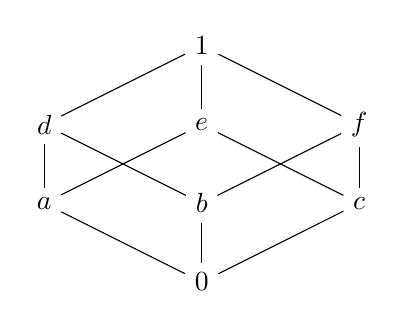
\begin{tikzpicture}[node distance=2cm]
        \node (top) at (0,0) {$1$};

        \node (a) at (-2,-2) {$a$};
        \node (b) at (0, -2) {$b$};
        \node (c) at (2, -2) {$c$};

        \node (d) at (-2, -1) {$d$}; 
        \node (e) at (0, -1) {$e$}; 
        \node (f) at (2, -1) {$f$}; 

        \node (bottom) at (0,-3) {$0$};

        \draw (bottom) -- (a); 
        \draw (bottom) -- (b); 
        \draw (bottom) -- (c);
        
        \draw (a) -- (e); 
        \draw (c) -- (e);

        \draw (a) -- (d); 
        \draw (b) -- (d);
        
        \draw (b) -- (f); 
        \draw (c) -- (f);

        \draw (d) -- (top); 
        \draw (e) -- (top); 
        \draw (f) -- (top);
        
    \end{tikzpicture}
\end{center}

\tableofcontents
\newpage
\section{Introduction}
\label{sec:Introduction}
\subsection{Lattices}
\label{subsec:Introduction-Lattices}
A lattice $\calC$ is a poset \st for any pair $(a,b) \in \calC$, the supremum $a \land b$, and infimum $a \lor b$ exist. We extend this to a complete lattice, which has the requirement that for any subset $\calD \subseteq \calC$ the supremum $\bigvee \calD$ and infimum $\bigwedge \calD$ exist. 

\subsection{Formal Contexts}
\label{subsec:Introduction-Formal_Contexts}
A Formal Context is a triple $\langle G, M, I \rangle$ where $G$ refers to a set of objects, $M$ to a set of properties, and $I$ an incidence relation over $G\times M$. 

We have derivation operators $A'$ and $B'$; for $A'$, where $A \subseteq G$, the derivation operator tells us which properties belong to the objects in $A$, the dual holds for properties and their objects. \textbf{Formally}, 

\begin{definition}
    \[ A' := \left\{m \in M \,|\, \forall g \in A, gIm\right\} \]
    \[ B' := \left\{g \in G \,|\, \forall m \in B, gIm\right\} \]
\end{definition}

We also have closure operators, $A''$, which works intuitively by applying the derivation operator on $A$ ($B$), which yields a set of properties. Then applying it again on $A'$ ($B'$), which yields back a set of objects (properties). 

\begin{proposition}
    For subsets $A, B\subseteq G$ (defined dually for properties $C,D \subseteq M$), we have
    \begin{itemize}
        \item[a.] $A \subseteq B \implies B' \subseteq A'$ 
        \item[b.] $A \subseteq A''$ 
        \item[c.] $A' = A'''$
    \end{itemize}
\end{proposition}

For more natural discussion, \textit{a} describes the behaviour that if we have two sets of objects $A$ and $B$, where $A \subseteq B$; then it follows that objects in $A$ will have at \textit{least} all the properties of objects in $B$. 

\subsection{Formal Concepts}
\label{sec:Introduction-Formal_Concepts}

\textit{Presume we are working with a formal context $\langle G, M, I \rangle$.}
\begin{definition}
    
    $(A,B)$ is a \textit{\textbf{formal concept}} of our formal context \textit{iff}    $A \subseteq G$, $B \subseteq M$, $A' = B$, and $B' = A$ 
\end{definition}

$A$ is called the \textbf{extent}, and $B$ is called the \textbf{intent}. We can refer to the set of all formal concepts of a formal context as a $\calB (G, M, I)$.

\end{document}
